%!TEX root = ../../dissertation.tex
%%%%%%%%%%%%%%%%%%%%%%%%%%%%%%%%%%%%%%%%%%%%%%%%%%%%%%%%%%%%%%%%%%%%%%%%%%%%%%%
\section{Modeling Mobile Network Load}
\label{c4:modeling}

Drawing conclusions from statistical analysis alone is a strenuous task. The next logical step lies therefore in the creation of models abstracting this real system, making them easier to calculate with the loss of some precision. This and future improved models should support network operators in predicting the signaling load in their core network with the benefit of improved network engineering and correctly scaling core components.

On the basis of the tunnel distributions attained in Section~\ref{c4:evaluations}, models for both a traditional \gls{GGSN} as well as a virtualized \gls{GGSN} are introduced. The performance trade-offs when using a virtual \gls{GGSN} are further studied, discussing different options to consider when using the virtual node.


%\cite{trangia-lbvs}

%%%%%%%%%%%%%%%%%%%%%%%%%%%%%%%%%%%%%%%%%%%%%%%%%%%%%%%%%%%%%%%%%%%%%%%%%%%%%%%
\subsection{Queuing Theory Basics}

To understand the modeling process some knowledge on queuing theory is required. The next few sections give a short overview on this.

\subsubsection{Little's Law}

A basic queuing system can be expressed as a stream of customers arriving at an arbitrary system with a rate $\lambda$. This system then processes the customers, taking an average time of $W$ on a number of processors until the customers depart again. On average $L$ customers will be in the system. The representation --- and queuing theory in general for that matter --- was originally devised for telephone networks by Erlang \cite{erlang1917solution}.

From that, Little's~Law~\cite{little1961proof} can be formulated as

\begin{equation}
\phantom{,}L = \lambda W\text{,}
\end{equation}

which holds universally independent of any specific arrival or service time process.

\subsubsection{Kendall's Notation}

To distinguish the variations of a queuing system's parameter a simple convention and naming scheme was devised by Kendall in in 1953 \cite{kendall1953stochastic} and later extended on.

In its simplest form the notation reads $A/S/s$ with $A$ denoting the arrival distribution, $S$ the service time, and $s$ the number of servers. Here, an extended notation will be used, 

\begin{equation}
A/S/s-q
\end{equation}

which additionally describes the queue length $q$. With this, a queuing system ($q=\infty$) can be easily distinguished from a blocking or loss system ($q=0$). The most commonly used arrival processes and service time distributions are summarized in Table~\ref{c4:tbl:kendalldistributions}.


\begin{table}[htbp]
	\caption{Typical abbreviation of processes in Kendall's notation.}
	\label{c4:tbl:kendalldistributions}
	\begin{tabu}{X[l]X[7]}
	\toprule
	\textbf{Symbol} & \textbf{Description} \\
	\midrule
	$M$ & Markovian, i.e. Poisson, arrival process or exponential service time distribution\\
	$D$ & Deterministic arrival process or service time distribution\\
	$G$ & General arrival process or service time distribution with no special assumptions\\
	$GI$ & General arrival process with independent arrivals; also called regenerative \\ 
	\bottomrule
	\end{tabu} 
\end{table}

\subsubsection{Information Gain}

Depending on the complexity of the specific queuing system model, much information can be gained. In simple cases the state probability can be mathematically determined, i.e. the probability, that exactly $m$ customers are in the system concurrently. If this number is higher than the number of processors, this also determines the queue length or the blocking probability $p_B$ if there is no queue. Other properties include for example the waiting time of customers.

\begin{figure}[htb]
	\centering
	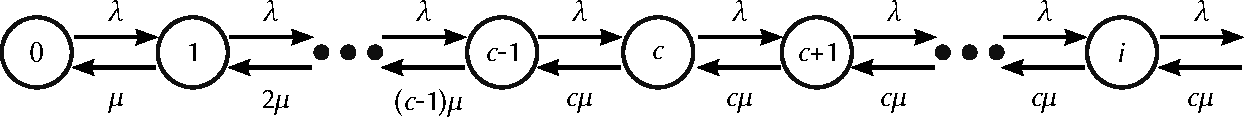
\includegraphics[width=\columnwidth]{images/markovchain.pdf}
	\caption{$M/M/n-\infty$ Markov chain model.}
	\label{c4:fig:markovchain}
\end{figure}

One such basic queuing system is $M/M/1-\infty$ \cite[pp.~94-99]{Kleinrock:1975:TVQ:1096491}, on which stationary analysis can be applied upon. Both the one processor queue and $M/M/n-\infty$ can also be easily expressed as a Markov chain due to their memoryless property. Figure~\ref{c4:fig:markovchain} depicts the state transitions of a system with $i$ processors and a queue length of $n-i$.

More complex models are often not tractable by stationary analysis or other mathematical tools anymore and no general solution is known. This is especially true for the class of $G/G/n$ systems, which can only be directly solved under certain conditions. A better approach can be the use of a queuing simulation. Hereby, both the arrival and the serving process are implemented in a \gls{DES} using random numbers of the desired distributions in order th ascertain the system load and blocking probability.

%%%%%%%%%%%%%%%%%%%%%%%%%%%%%%%%%%%%%%%%%%%%%%%%%%%%%%%%%%%%%%%%%%%%%%%%%%%%%%%
\subsection{Model Rationale}

One major metric to consider in the dimensioning is the number of supported tunnels, i.e. connections to the Internet, of the \gls{GGSN}.
The performance requirements of the \gls{GGSN} depend on factors like customers to serve, applications in the network, user behavior and devices used. These factors are, during dimensioning, either unknown or subject to change as user behavior evolves.

The latter adheres to the concept of \gls{NFV} \cite{nfv_whitepaper} suggesting to use technologies from cloud computing in the network. This would allow network operators to scale the node out instead of up. This means using additional low performance machines instead of completely replacing the existing \gls{GGSN} with a more powerful version. Today, these network components are typically sold in a static and monolithic form and can not be easily extended with of-the-shelf hardware in order to accommodate to a changing environment.


%%%%%%%%%%%%%%%%%%%%%%%%%%%%%%%%%%%%%%%%%%%%%%%%%%%%%%%%%%%%%%%%%%%%%%%%%%%%%%%
\subsection{Creating a Simple Toy Queuing Model}

\begin{figure}[htb]
	\centering
	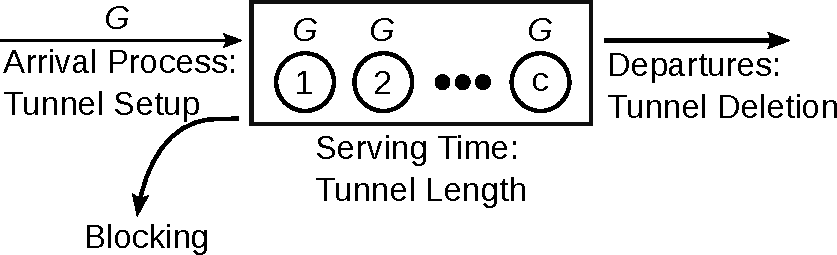
\includegraphics[width=\columnwidth]{images/GGn-model.pdf}
	\caption{Simple toy-model for tunnel-induced load on the core network.}
	\label{c4:fig:ggn-model}
\end{figure}

To begin the modeling process we attempt to represent the tunnel management as a queuing system, specifically as a G/G/n-0 system in Kendall's notation. Figure~\ref{c4:fig:ggn-model} shows this model for the case of our proposed tunnel load metric. Here, tunnels enter the system by a general random distribution, are then ``served'' at the \gls{GGSN} for the duration of their existence, which also follows a general distribution, and leave the system, i.e. are torn down, afterwards. If the serving units are filled, blocking occurs and arriving tunnel requests are rejected.

In this case ``servers'' correspond to available resources at one or more \gls{GGSN}, making the maximum number of tunnels hard to guess and depend on a number of factors. This could include soft-limits like the specific configuration, and hard-limits, e.g. the \gls{GGSN}'s processing and memory constraints. Unfortunately, all of these are unknown to us. Moreover, as the tunnels are all served on a relatively small number of hardware entities they are not independent of each other. Increasing load could very well influence both the arrival as well as the serving process.

For the purpose of creating a toy model we are further simplifying the $G/G/n-0$ to a $M/M/\infty$ queue. As stated, no actual limit to the number of virtual servers is known and the data also does not show any obvious limits. So we can safely assume an unlimited system and do not have to treat blocking or queuing explicitly.



Now, assuming both a Poisson arrival and an exponential serving process, a stationary analysis can be conducted. From the measured data an arrival rate of $\lambda=25.64123$ and the parameter $\mu=0.0001586728$ for the exponential service time distribution are calculated. Using Little's Law this gives an estimate for the mean number of concurrent tunnels at the \gls{GGSN} of 

$$
L=\frac{\lambda}{\mu}\approx 161\,599. %=161598.14.
$$

As stated, the amount of state held at the node and propagated through the network is directly related to the number of tunnels. Therefore, we propose this metric as an initial estimate of the load at the \gls{GGSN}.


%%%%%%%%%%%%%%%%%%%%%%%%%%%%%%%%%%%%%%%%%%%%%%%%%%%%%%%%%%%%%%%%%%%%%%%%%%%%%%%
\subsection{Advanced Models} 


On the basis of this toy model better fitting models can now be constructed. Those should also factor in more of the core network's properties and specified parameters omitted in this model. Specifically, this means shifting from $M/M/\infty$ to the more generalized $G/G/n$ and therefore finding better distribution fits for the involved processes.

It is also entirely possible that the single queue approach is not the best way to describe control plane load. Several load influencing factors discussed earlier have direct influence on the tunnel arrivals and duration, e.g. the device type or the radio access technology. Therefore, amongst others multidimensional queuing networks or fluid flow could be a better fit. Our plan is to conduct further investigations into the modeling of mobile core network signaling. This also includes a rough simulative approach, which could also be used to validate our models against experimental data.


%%
\subsubsection{Monolithic \texorpdfstring{\acrshort{GGSN}}{GGSN}}

In this section we provide a model for a traditional \gls{GGSN} and discuss a model for a virtual \gls{GGSN} using \gls{NFV}. In \gls{NFV} \cite{nfv_whitepaper} static network middleboxes are replaced by commodity hardware. The tasks solved by the original middleboxes are then solved by dediciated software.

\begin{figure}[htb]
  \centering
  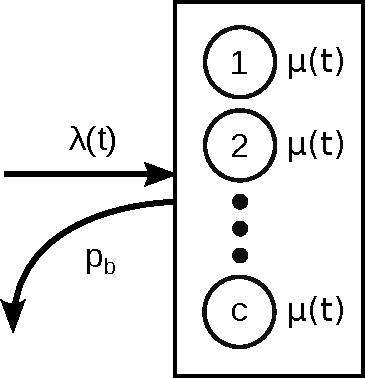
\includegraphics[width=0.6\textwidth]{images/ggsn-monolithic.pdf}
  \caption{Model of a Traditional GGSN}
  \label{fig:model_traditional_ggsn}
\end{figure}

First, we give a model for a \emph{traditional} \gls{GGSN}, i.e. a network static network component.
While we consider the \gls{GGSN} to be one fixed entity, it can in reality consist of multiple servers. However, due to the fact that the \gls{GGSN} is purchased from a vendor as a middlebox, idle servers can be neither deactivated nor reused for other purposes.

The queuing theory equivalent is displayed in Figure~\ref{fig:model_traditional_ggsn}. New tunnels requests arrive according to a Poisson distribution with a rate of $\lambda(t)$ at the \gls{GGSN}. This server will have a maximum tunnel capacity of $c_c$. When it is reached, blocking will occur and newly incoming tunnels are rejected. Traditionally, \glspl{GGSN} can be expected to be overdimensioned in such a way, that this rarely happens. If the new tunnel is accepted, it will occupy one of the serving units of the unit for the duration $\mu(t)$ of the tunnel. As stated earlier, we can not model the tunnel duration to be markovian, resulting in a  $M/G/c_c$ loss system. In order to give quality of service guarantees the network operator is interested in the system's blocking probability $p_B$, which we consider to be a key metric of our model. Additionally, the previously described diurnal patterns can are also be modeled by adjusting the arrival and serving process distributions for each time of day. This alternatively also allows just to investigate the busy hour and thus the system's peak load.


%%
\subsubsection{\texorpdfstring{\acrshort{GGSN}}{GGSN} using Network Function Virtualization}
\label{c4:sec:virtual_ggsn}

\begin{figure}[htb]
  \centering
  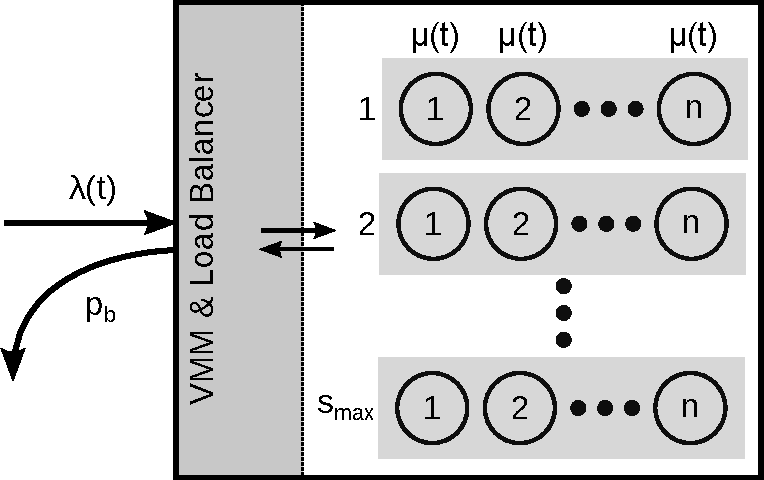
\includegraphics[width=0.7\textwidth]{images/ggsn-virtualized.pdf}
  \caption{Model of a GGSN using Network Function Virtualization}
  \label{c4:fig:model_nfv_ggsn}
\end{figure}

In the second model, we introduce concepts from \gls{NFV}, i.e. the idea to replace middleboxes with commodity hardware. This allows us to realize benefits from cloud computing, as we are now able to scale out, instead of up. The assumptions of the Markov arrival process $\lambda(t)$ and the serving time distributions $\mu(t)$ are carried over. However, instead of one server processing every tunnel, this model assumes that there are up to $s_{max}$ virtualized servers $s_i$. Each of these is much smaller than the traditional \gls{GGSN}, having a tunnel serving capacity of $c_i \ll c_c$ and a total system capacity of $c_{max} = s_{max} \times i$.

In its initial state, for efficiency, all but a small portion of the server instances should be shut of. Only, when a certain condition is reached, a new one is provisioned. As a simple example, one could always hold one instance in reserve for upcoming requests and provision as soon as the reserver gets used. Similar rules should apply in the shutdown of servers and should form a hysteresis together with the boot condition. For example it would be possible to keep at least one server in reserve but never more than two.

If these conditions are not carefully selected and are in tune with the expected boot time of an instance, additional blocking can occur. Despite not having reached its maximum capacity, this system will still reject tunnel requests during the provisioning phase when no tunnel slots are free. This could be remedied by a request queue. However, this might just make the system more complex without providing real benefit, as mobile devices usually will repeat their attempts and would time out anyway when the request is taking too long. 

To place incoming tunnel state on one of the available servers a load balancer is required. To ensure, that the system in run time can scale down to its actual needs, the balancer should place tunnels on servers, that are the fullest, keeping the reserve free. It may even migrate tunnel state from almost empty servers away so that these can be shut down, when the condition is fulfilled. Keeping instance close to their capacity should also have no impact on the performance a mobile device associated to a specific tunnel experiences. Adequate strategies for both load balancing and migration will be considered in future work.



